%%%%%%%%%%%%%%%%%%%%%%%%%%%%%%%%%%%%%%%%%%%%%%%%%%%%%%%%%%%%%%%%%%%%%%%%%%%%%%%%%
%% Documenclass 
%%%%%%%%%%%%%%%%%%%%%%%%%%%%%%%%%%%%%%%%%%%%%%%%%%%%%%%%%%%%%%%%%%%%%%%%%%%%%%%%%
\documentclass[a4paper,oneside,titlepage]{report}
%%%%%%%%%%%%%%%%%%%%%%%%%%%%%%%%%%%%%%%%%%%%%%%%%%%%%%%%%%%%%%%%%%%%%%%%%%%%%%%%%
%% Packages
%%%%%%%%%%%%%%%%%%%%%%%%%%%%%%%%%%%%%%%%%%%%%%%%%%%%%%%%%%%%%%%%%%%%%%%%%%%%%%%%%
\usepackage{tabularx} % Paquete para tablas de ancho ajustable
\usepackage{array}    % Paquete para personalizar columnas
\usepackage{enumitem}
\usepackage[english]{babel}
\usepackage{amsmath}
\usepackage{complexity}
\usepackage[T1]{fontenc}
\usepackage[utf8]{inputenc}
\usepackage[pdftex]{graphicx} %%Graphics in pdfLaTeX
\usepackage{graphicx}
\usepackage[font=bf, labelsep=endash]{caption} 
\usepackage{a4wide} %%Smaller margins, more text per page.
\usepackage{longtable} %%For tables that exceed a page width
\usepackage{pdflscape} %%Adds PDF sup­port to the land­scape en­vi­ron­ment of pack­age
\usepackage{caption} %%Pro­vides many ways to cus­tomise the cap­tions in float­ing en­vi­ron­ments like fig­ure and ta­ble
\usepackage{float} %%Im­proves the in­ter­face for defin­ing float­ing ob­jects such as fig­ures and ta­bles
\usepackage[tablegrid,nochapter]{vhistory} %%Vhis­tory sim­pli­fies the cre­ation of a his­tory of ver­sions of a doc­u­ment
\usepackage[nottoc]{tocbibind} %%Au­to­mat­i­cally adds the bib­li­og­ra­phy and/or the in­dex and/or the con­tents, etc., to the Ta­ble of Con­tents list­ing
\usepackage[toc,page]{appendix} %%The ap­pendix pack­age pro­vides var­i­ous ways of for­mat­ting the ti­tles of ap­pen­dices
\usepackage{pdfpages} %%This pack­age sim­pli­fies the in­clu­sion of ex­ter­nal multi-page PDF doc­u­ments in LATEX doc­u­ments
\usepackage[rightcaption]{sidecap} %%De­fines en­vi­ron­ments called SC­fig­ure and SCtable (anal­o­gous to fig­ure and ta­ble) to type­set cap­tions side­ways
\usepackage{cite} %%The pack­age sup­ports com­pressed, sorted lists of nu­mer­i­cal ci­ta­tions, and also deals with var­i­ous punc­tu­a­tion and other is­sues of rep­re­sen­ta­tion, in­clud­ing com­pre­hen­sive man­age­ment of break points
\usepackage[]{acronym} %%This pack­age en­sures that all acronyms used in the text are spelled out in full at least once. It also pro­vides an en­vi­ron­ment to build a list of acronyms used
\usepackage[pdftex,scale={.8,.8}]{geometry} %%The pack­age pro­vides an easy and flex­i­ble user in­ter­face to cus­tomize page lay­out, im­ple­ment­ing auto-cen­ter­ing and auto-bal­anc­ing mech­a­nisms so that the users have only to give the least de­scrip­tion for the page lay­out. For ex­am­ple, if you want to set each mar­gin 2cm with­out header space, what you need is just \usep­a­ck­age[mar­gin=2cm,no­head]{ge­om­e­try}.
\usepackage{layout} %%The pack­age de­fines a com­mand \lay­out, which will show a sum­mary of the lay­out of the cur­rent doc­u­ment
%\usepackage{subcaption}
%\usepackage{subfigure} %%Pro­vides sup­port for the ma­nip­u­la­tion and ref­er­ence of small or ‘sub’ fig­ures and ta­bles within a sin­gle fig­ure or ta­ble en­vi­ron­ment.
\usepackage[toc]{glossaries} %%The glos­saries pack­age sup­ports acronyms and mul­ti­ple glos­saries, and has pro­vi­sion for op­er­a­tion in sev­eral lan­guages (us­ing the fa­cil­i­ties of ei­ther ba­bel or poly­glos­sia).
\usepackage[left,pagewise,modulo]{lineno} %%Adds line num­bers to se­lected para­graphs with ref­er­ence pos­si­ble through the LATEX \ref and \pageref cross ref­er­ence mech­a­nism
\usepackage[pdftex,colorlinks=false,hidelinks,pdfstartview=FitV]{hyperref}%%The hy­per­ref pack­age is used to han­dle cross-ref­er­enc­ing com­mands in LATEX to pro­duce hy­per­text links in the doc­u­ment. 
\usepackage{metainfo}
\usepackage[raggedright]{titlesec}
\usepackage{titleps}
\usepackage{etoolbox}
\usepackage{bookmark}
\usepackage{%
	array, %%An ex­tended im­ple­men­ta­tion of the ar­ray and tab­u­lar en­vi­ron­ments which ex­tends the op­tions for col­umn for­mats, and pro­vides "pro­grammable" for­mat spec­i­fi­ca­tions
	booktabs, %%The pack­age en­hances the qual­ity of ta­bles in LATEX, pro­vid­ing ex­tra com­mands as well as be­hind-the-scenes op­ti­mi­sa­tion
	dcolumn, %%
	rotating,
	shortvrb,
	units,
	url,
	lastpage,
	longtable,
	lscape,
	qtree,
	skmath,	
}
\usepackage{tocloft}
%%%%%%%%%%%%%%%%%%%%%%%%%%%%%%%%%%%%%%%%%%%%%%%%%%%%%%%%%%%%%%%%%%%%%%%%%%%%%%%%%
%% Java --> latex 
%%%%%%%%%%%%%%%%%%%%%%%%%%%%%%%%%%%%%%%%%%%%%%%%%%%%%%%%%%%%%%%%%%%%%%%%%%%%%%%%%
\usepackage{listings}
\usepackage{color}
\definecolor{pblue}{rgb}{0.13,0.13,1}
\definecolor{pgreen}{rgb}{0,0.5,0}
\definecolor{pred}{rgb}{0.9,0,0}
\definecolor{pgrey}{rgb}{0.46,0.45,0.48}
\usepackage{inconsolata}
\input{base/javainputstyle}
%%%%%%%%%%%%%%%%%%%%%%%%%%%%%%%%%%%%%%%%%%%%%%%%%%%%%%%%%%%%%%%%%%%%%%%%%%%%%%%%%
\setlength{\parindent}{0pt}
\setlength{\parskip}{.5\baselineskip}
%%%%%%%%%%%%%%%%%%%%%%%%%%%%%%%%%%%%%%%%%%%%%%%%%%%%%%%%%%%%%%%%%%%%%%%%%%%%%%%%%
%% Inserting the metadata
%%%%%%%%%%%%%%%%%%%%%%%%%%%%%%%%%%%%%%%%%%%%%%%%%%%%%%%%%%%%%%%%%%%%%%%%%%%%%%%%%
% !TeX root = ../alda_g17.tex

\def\BoldTitle{Informe \#1}

\def\Subtitle{Definición del problema}

\def\Authors{Integrantes:\\ 
Owuen Yagual Panimboza \\ 
Stiven Rivera Palma}

\def\Logo{./images/logo_espol2.png}

%%%%%%%%%%%%%%%%%%%%%%%%%%%%%%%%%%%%%%%%%%%%%%%%%%%%%%%%%%%%%%%%%%%%%%%%%%%%%%%%%
%% Creating the frontpage
%%%%%%%%%%%%%%%%%%%%%%%%%%%%%%%%%%%%%%%%%%%%%%%%%%%%%%%%%%%%%%%%%%%%%%%%%%%%%%%%%
\AtBeginDocument{

\begin{titlepage}
\centering

{\Huge \textbf{\BoldTitle} \par}

\vspace{0.5cm}

{\Large \Subtitle \par}

\vspace{1.5cm}

\includegraphics[width=0.8\textwidth]{\Logo}

\vspace{1.5cm}

{\large \Authors \par}

\vfill

12 de Junio, 2026

\end{titlepage}

}

%%%%%%%%%%%%%%%%%%%%%%%%%%%%%%%%%%%%%%%%%%%%%%%%%%%%%%%%%%%%%%%%%%%%%%%%%%%%%%%%%
%% Creation of the header
%%%%%%%%%%%%%%%%%%%%%%%%%%%%%%%%%%%%%%%%%%%%%%%%%%%%%%%%%%%%%%%%%%%%%%%%%%%%%%%%%
\patchcmd{\chapter}{plain}{short}{}{} %$ <-- the header on chapter 1
%%%%%%%%%%%%%%%%%%%%%%%%%%%%%%%%%%%%%%%%%%%%%%%%%%%%%%%%%%%%%%%%%%%%%%%%%%%%%%%%%
%% Creation of page-styles
%%%%%%%%%%%%%%%%%%%%%%%%%%%%%%%%%%%%%%%%%%%%%%%%%%%%%%%%%%%%%%%%%%%%%%%%%%%%%%%%%
\newpagestyle{long}{
  \sethead
    [\thepage]
    []
    [\chaptername\ \thechapter:\ \chaptertitle]
    {\chaptername\ \thechapter:\ \chaptertitle}
    {}
    {\thepage}

  \headrule
}

\newpagestyle{short}{
  \sethead
    [\thepage]
    []
    []
    {}
    {}
    {\thepage}

  \headrule
}
%%%%%%%%%%%%%%%%%%%%%%%%%%%%%%%%%%%%%%%%%%%%%%%%%%%%%%%%%%%%%%%%%%%%%%%%%%%%%%%%%
%% DOCUMENT
%%%%%%%%%%%%%%%%%%%%%%%%%%%%%%%%%%%%%%%%%%%%%%%%%%%%%%%%%%%%%%%%%%%%%%%%%%%%%%%%%
\renewcommand{\thefigure}{\arabic{figure}.} 
\renewcommand{\figurename}{Figure}
\renewcommand{\cftfigpresnum}{\figurename~}
\setlength{\cftfigindent}{0em}
\setlength{\cftfignumwidth}{5em}
\renewcommand{\thetable}{\arabic{table}.}
\renewcommand{\tablename}{Table}
\renewcommand{\cfttabpresnum}{\tablename~} 
\setlength{\cfttabindent}{0em}
\setlength{\cfttabnumwidth}{5em}

\begin{document}

\pagenumbering{roman}
\DeclareGraphicsExtensions{.pdf,.jpg,.png}
\pagestyle{short}

\newpage
%%%%%%%%%%%%%%%%%%%%%%%%%%%%%%%%%%%%%%%%%%%%%%%%%%%%%%%%%%%%%%%%%%%%%%%%%%%%%%%%%
%% Table of contents
%%%%%%%%%%%%%%%%%%%%%%%%%%%%%%%%%%%%%%%%%%%%%%%%%%%%%%%%%%%%%%%%%%%%%%%%%%%%%%%%%

\pagestyle{long}




%%%%%%%%%%%%%%%%%%%%%%%%%%%%%%%%%%%%%%%%%%%%%%%%%%%%%%%%%%%%%%%%%%%%%%%%%%%%%%%%%
%% Version table insertion
%%%%%%%%%%%%%%%%%%%%%%%%%%%%%%%%%%%%%%%%%%%%%%%%%%%%%%%%%%%%%%%%%%%%%%%%%%%%%%%%%
%\input{base/history}
\pagenumbering{arabic}
%%%%%%%%%%%%%%%%%%%%%%%%%%%%%%%%%%%%%%%%%%%%%%%%%%%%%%%%%%%%%%%%%%%%%%%%%%%%%%%%%
%% Inserting all the content
%%%%%%%%%%%%%%%%%%%%%%%%%%%%%%%%%%%%%%%%%%%%%%%%%%%%%%%%%%%%%%%%%%%%%%%%%%%%%%%%%
% !TeX root = ../alda_g17.tex

\tableofcontents

\chapter{Introduction}

\section{Descripción del problema}
La captura de movimiento markerless (sin marcadores físicos) representa una línea activa de investigación en visión artificial con aplicaciones en robótica, rehabilitación médica, interfaces humano-máquina e interacción natural. \cite{Pauzietal2021}

Los enfoques tradicionales basados en sensores físicos, trajes de captura óptica o cámaras de profundidad resultan costosos e intrusivos. El presente proyecto propone un sistema basado exclusivamente en una cámara convencional que, procesando el video en tiempo real, detecte la pose del brazo humano, calcule los ángulos articulares de hombro, codo y muñeca, y transfiera esos valores a la simulación visual de un brazo robótico virtual de tres grados de libertad (GDL).  \cite{Vintimilla2026}

La solución adopta MediaPipe Pose de Google, un framework de código abierto que proporciona detección de 33 landmarks corporales en tiempo real sin necesidad de GPU, combinado con OpenCV para la adquisición y el procesamiento de imagen. \cite{Bazarevskyetal2020} \cite{Lugaresietal2019}

\subsection*{Diagrama de Bloques General del Sistema}
La figura \ref{fig:diagrama_bloques} representa el flujo de datos global del proyecto, descompuesto en sus cinco módulos funcionales principales.

\begin{figure}[h!]
    \centering
    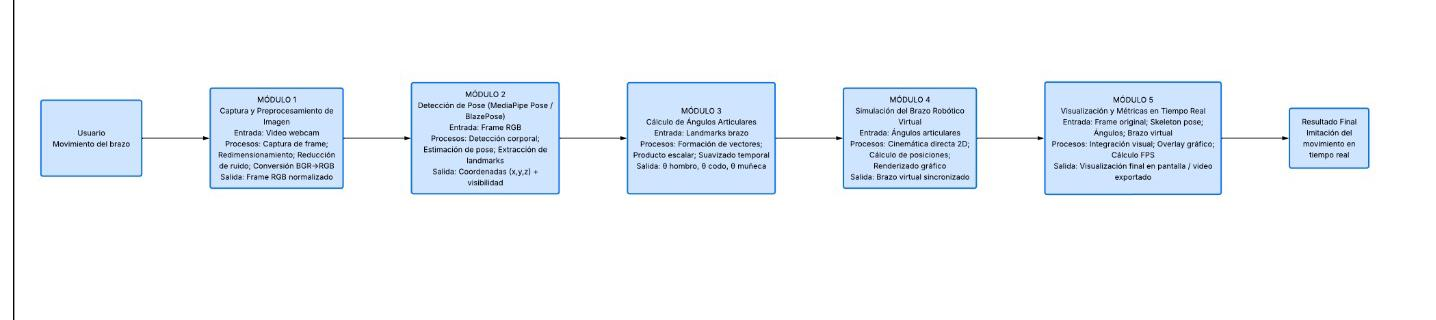
\includegraphics[width=1\textwidth]{images/diagrama_bloques.jpeg}
    \caption{Diagrama de bloques del sistema de imitación de movimientos con MediaPipe Pose.}
    \label{fig:diagrama_bloques}
\end{figure}

Cada bloque representa un módulo funcional independiente con entradas y salidas definidas. El video de la cámara entra al sistema por M1, los landmarks son extraídos en M2, los ángulos se calculan en M3, el brazo robótico es simulado en M4 y todo se integra visualmente en M5. \cite{Bazarevskyetal2020} \cite{Bradski2000}
\section{Justificación del problema}
MediaPipe fue presentado originalmente como un framework modular para construir pipelines de percepción reproducibles entre plataformas. Su componente BlazePose amplió esta capacidad al dominio de la estimación de pose corporal en tiempo real, logrando latencias menores a 30 ms en CPU mediante un pipeline de dos etapas: detector de persona (BlazePose Detector) y estimador de pose (BlazePose Estimator) que extrae 33 puntos clave. \cite{Bazarevskyetal2020} \cite{Lugaresietal2019}

Trabajos previos como los de Pauzi et al. (2021) demostraron la efectividad de BlazePose para estimar movimientos corporales con una diferencia de precisión dentro del 10\% respecto a sistemas IMU de referencia. En el dominio de la teleoperación robótica, Altayeb (2023) implementó un sistema de replicación de gestos de mano en un brazo robótico usando MediaPipe Hands, validando la viabilidad de este enfoque para control de actuadores virtuales. \cite{Pauzietal2021} \cite{Altayeb2023}

La justificación económica radica en el bajo costo de implementación: el sistema requiere únicamente una webcam USB estándar ($<$ \$20 USD), sin sensores de profundidad ni hardware especializado. El stack de software es completamente open-source (Python, OpenCV, MediaPipe, NumPy).

\section{Objetivos}

\subsection{Objetivo principal}
Desarrollar un sistema de visión artificial que, a partir de video capturado en tiempo real por una cámara convencional, detecte los movimientos del brazo humano utilizando MediaPipe Pose \cite{Bazarevskyetal2020} \cite{Lugaresietal2019}, calcule los ángulos de las articulaciones hombro, codo y muñeca, y los transfiera a la simulación visual sincronizada de un brazo robótico virtual de 3 GDL.

\subsection{Objetivos específicos}
\begin{enumerate}
    \item Implementar un módulo de captura y preprocesamiento de video en tiempo real usando OpenCV \cite{Bradski2000} con soporte para normalización de resolución (640×480) y conversión de espacio de color BGR→RGB.
    \item Integrar el modelo MediaPipe Pose \cite{Bazarevskyetal2020} para la detección y extracción de los 33 landmarks corporales, con énfasis en los puntos clave del brazo (hombros: landmarks 11,12; codos: 13,14; muñecas: 15,16).
    \item Desarrollar un módulo de cálculo de ángulos articulares mediante álgebra vectorial (producto escalar y norma de vectores) para los tres GDL del brazo: hombro (elevación), codo (flexión) y muñeca (flexión), con filtrado de media móvil de 5 frames.
    \item Implementar la simulación 2D del brazo robótico virtual mediante cinemática directa, renderizando en tiempo real el modelo sobre el frame de video usando primitivas OpenCV (cv2.line, cv2.circle) \cite{Bradski2000}.
    \item Construir un módulo de visualización integrada que muestre el skeleton de MediaPipe \cite{Lugaresietal2019}, los ángulos articulares calculados, el brazo robótico simulado y métricas de rendimiento (FPS).
    \item Evaluar el desempeño del sistema con métricas de latencia (FPS objetivo: $\geq$ 20 FPS), precisión angular y estabilidad del sistema ante variaciones de iluminación, usando como referencia el benchmark del dataset COCO Keypoints \cite{10.1007/978-3-319-10602-1_48}.
\end{enumerate}

\section{Módulos del proyecto}
El sistema se descompone en cinco módulos funcionales interconectados. La arquitectura modular facilita el desarrollo y prueba independiente de cada componente en el marco SCRUM adoptado. Las tecnologías principales son OpenCV \cite{Bradski2000} para procesamiento de imagen y MediaPipe Pose \cite{Bazarevskyetal2020, 10.1007/978-3-319-10602-1_48} para estimación de pose.

\subsection{Módulo 1 -- Captura y Preprocesamiento de Imagen}

\subsubsection*{Objetivo}
Adquirir el flujo de video en tiempo real desde la cámara y preparar
cada frame para su procesamiento posterior mediante normalización de
resolución, conversión de espacio de color y reducción de ruido.

\paragraph{Entradas y Salidas}

\begin{table}[h!]
\centering
\label{tab:m1_io}
\renewcommand{\arraystretch}{1.3}
\begin{tabularx}{\textwidth}{
    >{\bfseries}p{3cm}
    X
    X
}    
\toprule
&
\textbf{Descripción} &
\textbf{Formato / Especificación} \\
\midrule
Entrada &
  Flujo de video desde webcam USB o cámara integrada &
  Resolución variable (640$\times$480 -- 1920$\times$1080), 30~FPS \\
\midrule
Salida &
  Frame de imagen normalizado en espacio RGB &
  NumPy array RGB, resolución fija 640$\times$480, píxeles en $[0,\,255]$ \\
\bottomrule
\end{tabularx}
\caption{Entradas y salidas del Módulo 1.}
\end{table}

\paragraph{Herramientas Tecnológicas}
\begin{itemize}[leftmargin=1.5em]
  \item \textbf{Software:} Python~3.10+ como lenguaje de implementación.
  \item \textbf{Librería principal:} OpenCV (cv2~v4.8+) \cite{Bradski2000}
        — captura de video (cv2.VideoCapture), redimensionado
        (cv2.resize) y conversión de espacio de color
        (cv2.cvtColor).
  \item \textbf{Librería de soporte:} NumPy (v1.24+) para manejo
        y operaciones sobre arrays de imagen.
\end{itemize}

\paragraph{Técnicas de Visión Computacional}
\begin{itemize}[leftmargin=1.5em]
  \item \textbf{Realzado y restauración:} aplicación opcional de filtro
        gaussiano (cv2.GaussianBlur) para atenuación de ruido
        de alta frecuencia antes de la inferencia de
        MediaPipe~\cite{GonzalezWoods2018}.
  \item Redimensionado con interpolación bicúbica
        (cv2.INTER\_CUBIC) para preservar calidad de bordes
        al escalar el frame.
  \item Conversión de espacio de color BGR$\to$RGB requerida por el
        modelo BlazePose de MediaPipe.
\end{itemize}

\subsection{Módulo 2 -- Detección de Pose con MediaPipe}
\subsubsection*{Objetivo}

Detectar los 33~landmarks del cuerpo humano en cada frame de video
utilizando el modelo MediaPipe~Pose (BlazePose), con énfasis en los
puntos clave del brazo: hombros (landmarks~11,~12), codos
(13,~14) y muñecas (15,~16)~\cite{Bazarevskyetal2020}.

\subsubsection*{Entradas y Salidas}

\begin{table}[h!]
\centering
\label{tab:m1_io}
\renewcommand{\arraystretch}{1.3}
\begin{tabularx}{\textwidth}{
    >{\bfseries}p{3cm}
    X
    X
}    
\toprule
&
\textbf{Descripción} &
\textbf{Formato / Especificación} \\
\midrule
Entrada &
  Frame RGB preprocesado (salida de M1) &
  NumPy array RGB 640$\times$480 \\
\midrule
Salida &
  33~landmarks corporales con visibilidad &
  \texttt{NormalizedLandmarkList}: coord.\
  $(x,\,y,\,z) \in [0,1]$ + visibilidad $\in [0,1]$
  por punto \\
\bottomrule
\end{tabularx}
\caption{Entradas y salidas del Módulo 2.}
\end{table}
 
\paragraph{Herramientas Tecnológicas}
\begin{itemize}[leftmargin=1.5em]
  \item \textbf{Modelo de IA preentrenado:}
        MediaPipe~Pose (BlazePose)~v0.10+~\cite{Bazarevskyetal2020,Lugaresietal2019}
        — modelo de estimación de pose de 33~landmarks entrenado sobre
        el dataset COCO~Keypoints. No requiere GPU.
  \item \textbf{Framework:} MediaPipe (Google) \cite{Lugaresietal2019}
        — framework de construcción de pipelines de percepción con
        soporte cross-platform.
  \item \textbf{Librería de soporte:} NumPy para extracción y
        transformación de las coordenadas de landmarks al espacio de
        píxeles.
\end{itemize}
 
\paragraph{Técnicas de Visión Computacional}
\begin{itemize}[leftmargin=1.5em]
  \item \textbf{Pipeline BlazePose de dos etapas:}
        \begin{enumerate}[leftmargin=2em]
          \item Detector de persona que delimita el bounding
                box de la región de interés.
          \item Estimador de pose que infiere los 33 landmarks con
                alta precisión dentro de esa región.
        \end{enumerate}
  \item \textbf{Modo de video} (static\_image\_mode=False):
        el modelo aprovecha la coherencia temporal entre frames
        consecutivos para acelerar la inferencia y estabilizar los
        landmarks.
  \item \textbf{Extracción de landmarks de interés:} se seleccionan los
        índices 11–16 (hombros, codos, muñecas) de los 33~puntos
        detectados para alimentar el módulo de cálculo angular.
\end{itemize}

\subsection{Módulo 3 -- Cálculo de Ángulos Articulares}
\subsubsection*{Objetivo}
Calcular los ángulos de flexión/extensión en las articulaciones
hombro, codo y muñeca a partir de las coordenadas 2D de los landmarks,
usando la definición vectorial del ángulo entre dos segmentos
articulares.

\subsubsection*{Entradas y Salidas}

\begin{table}[h!]
\centering
\label{tab:m1_io}
\renewcommand{\arraystretch}{1.3}
\begin{tabularx}{\textwidth}{
    >{\bfseries}p{3cm}
    X
    X
}    
\toprule
&
\textbf{Descripción} &
\textbf{Formato / Especificación} \\
\midrule
Entrada &
  Coordenadas 2D de hombro, codo y muñeca (salida de M2) &
  Pares $(x,\,y)$ en píxeles para cada articulación
  (landmarks 11–16) \\
\midrule
Salida &
  Tripleta de ángulos articulares suavizados &
  $\theta_{\text{hombro}},\,\theta_{\text{codo}},\,
   \theta_{\text{muñeca}}$ en grados $[0°,\,180°]$ (float64) \\
\bottomrule
\end{tabularx}
\caption{Entradas y salidas del Módulo 3.}
\end{table}

\paragraph{Herramientas Tecnológicas}\mbox{}

\begin{itemize}[leftmargin=1.5em]
  \item \textbf{Librería principal:} NumPy (v1.24+) para
        cálculo del producto escalar (np.dot), norma de
        vectores (np.linalg.norm) y función
        arccos (np.arccos) necesarios en la fórmula
        angular.
  \item \textbf{Librería de soporte:} Matplotlib (v3.7+)
        para graficar la evolución temporal de los ángulos articulares
        durante las pruebas y análisis de resultados.
\end{itemize}
 
\paragraph{Técnicas de Visión Computacional y Geometría}
\begin{itemize}[leftmargin=1.5em]
  \item \textbf{Cálculo de ángulos mediante producto escalar:}
        \cite{GonzalezWoods2018}
 
        \begin{equation}
            \theta \;=\; \arccos{ \frac{\vec{v}_1 \cdot \vec{v}_2}{|\vec{v}_1|\,|\vec{v}_2|} }
            \label{eq:angulo}
        \end{equation}

        donde $\vec{v}_1$ y $\vec{v}_2$ son los vectores que forman
        cada par de segmentos en la articulación.

  \item \textbf{Filtrado temporal con media móvil} de ventana $w = 5$
        frames para suavizar fluctuaciones por ruido de detección de
        BlazePose y evitar movimientos bruscos en la simulación del
        brazo robótico.
  \item \textbf{Cálculo de vectores entre articulaciones:} diferencia
        de coordenadas entre el landmark proximal y el distal para
        construir cada vector de segmento corporal.
\end{itemize}
 

\subsection{Módulo 4 -- Simulación del Brazo Robótico Virtual}

\subsubsection*{Objetivo}
Representar y animar en pantalla un brazo robótico de 3~GDL cuyas
posiciones articulares se corresponden directamente con los ángulos
calculados por M3, logrando una imitación visual sincronizada en
tiempo real~\cite{Altayeb2023}.

\subsubsection*{Entradas y Salidas}

\begin{table}[h!]
\centering
\label{tab:m1_io}
\renewcommand{\arraystretch}{1.3}
\begin{tabularx}{\textwidth}{
    >{\bfseries}p{3cm}
    X
    X
}    
\toprule
&
\textbf{Descripción} &
\textbf{Formato / Especificación} \\
\midrule
Entrada &
  Ángulos articulares suavizados (salida de M3) &
  $\theta_{\text{hombro}},\,\theta_{\text{codo}},\,
   \theta_{\text{muñeca}}$ en grados (float64) \\
\midrule
Salida &
  Frame con overlay del brazo robótico virtual &
  NumPy array BGR con eslabones y articulaciones renderizados
  en tiempo real \\
\bottomrule
\end{tabularx}
\caption{Entradas y salidas del Módulo 4.}
\end{table}
 
\paragraph{Herramientas Tecnológicas}
\begin{itemize}[leftmargin=1.5em]
  \item \textbf{Librería principal:}
        OpenCV (cv2)~\cite{Bradski2000} para renderizado
        de primitivas gráficas: cv2.line (eslabones),
        cv2.circle (articulaciones),
        cv2.putText (ángulos).
  \item \textbf{Librería de soporte:} NumPy para el cálculo
        de coordenadas cartesianas de cada articulación mediante
        cinemática directa 2D.
\end{itemize}

\paragraph{Técnicas de Visión Computacional y Robótica}
\begin{itemize}[leftmargin=1.5em]
  \item \textbf{Cinemática directa 2D:} a partir de los ángulos
        articulares y las longitudes de eslabón predefinidas
        ($L_{\text{hombro}}$, $L_{\text{antebrazo}}$,
        $L_{\text{mano}}$), se calculan las posiciones cartesianas
        $(x,\,y)$ de cada junta del brazo virtual mediante relaciones
        trigonométricas acumulativas:
 
        \begin{align}
          x_1 &= x_0 + L_{\text{hombro}}\cos(\theta_{\text{hombro}})
          \notag \\
          y_1 &= y_0 - L_{\text{hombro}}\sin(\theta_{\text{hombro}})
          \notag \\
          x_2 &= x_1 + L_{\text{antebrazo}}
                        \cos(\theta_{\text{hombro}}
                             + \theta_{\text{codo}})
          \notag \\
          y_2 &= y_1 - L_{\text{antebrazo}}
                        \sin(\theta_{\text{hombro}}
                             + \theta_{\text{codo}})
          \label{eq:cinematica}
        \end{align}
 
  \item \textbf{Renderizado de overlay:} el brazo robótico se
        dibuja sobre el frame de video como una capa superpuesta,
        permitiendo la comparación visual directa entre el movimiento
        humano y la imitación del brazo virtual.
\end{itemize}

\subsection{Módulo 5 -- Visualización y Métricas en Tiempo Real}

\subsubsection*{Objetivo}
Integrar y mostrar en una ventana unificada el frame original anotado
con el skeleton de MediaPipe, los ángulos calculados, el
brazo robótico virtual y las métricas de rendimiento del sistema
(FPS).

\subsubsection*{Entradas y Salidas}

\begin{table}[h!]
\centering
\label{tab:m1_io}
\renewcommand{\arraystretch}{1.3}
\begin{tabularx}{\textwidth}{
    >{\bfseries}p{3cm}
    X
    X
}    
\toprule
&
\textbf{Descripción} &
\textbf{Formato / Especificación} \\
\midrule
Entrada &
  Frame original $+$ landmarks $+$ ángulos $+$
  overlay del brazo robótico &
  Salidas de M1, M2, M3 y M4 en cada iteración del
  bucle principal \\
\midrule
Salida &
  Frame anotado final visualizado en tiempo real &
  Ventana OpenCV (cv2.imshow) con overlay
  completo; exportación opcional a MP4
  (cv2.VideoWriter) \\
\bottomrule
\end{tabularx}
\caption{Entradas y salidas del Módulo 5.}
\end{table}
 
\paragraph{Herramientas Tecnológicas}
\begin{itemize}[leftmargin=1.5em]
  \item \textbf{Librería principal:}
        OpenCV (cv2)~\cite{Bradski2000} — visualización
        en ventana interactiva (cv2.imshow,
        cv2.waitKey) y exportación de video
        (cv2.VideoWriter).
  \item \textbf{MediaPipe Drawing Utils}~\cite{Lugaresietal2019}
        — dibujo automático del skeleton de 33~landmarks y
        conexiones corporales sobre el frame.
  \item Matplotlib (v3.7+) — generación de gráficas de
        evolución temporal de ángulos articulares y métricas de FPS
        para análisis de resultados.
  \item scikit-learn (v1.3+) — cálculo de métricas
        estadísticas de evaluación: error medio angular (MAE),
        correlación de Pearson y análisis de estabilidad del sistema.
\end{itemize}
 
\paragraph{Técnicas de Visión Computacional}
\begin{itemize}[leftmargin=1.5em]
  \item \textbf{Cálculo de FPS en tiempo real:} medición del tiempo
        de procesamiento por frame con timestamps de Python
        (time.time()) para monitoreo continuo del rendimiento
        del sistema.
  \item \textbf{Visualización compuesta:} superposición de múltiples
        capas (frame original, skeleton MediaPipe,
        overlay robótico, texto de métricas) mediante
        operaciones de blendingde OpenCV.
\end{itemize}

\section{Soluciones existentes}

Hoy en día, replicar los movimientos del cuerpo humano mediante visión por computadora es un campo clave para disciplinas como la robótica, la interacción persona-ordenador, la medicina de rehabilitación y la automatización. En la literatura actual encontramos diferentes estrategias para resolver esto, pero casi todas comparten el mismo fin: capturar lo que hace un usuario, calcular dónde están sus articulaciones en el espacio y trasladar esa información a un robot o a un entorno digital.

Una de las líneas de investigación con más fuerza es la teleoperación por imitación. Aquí el reto principal no es solo registrar el movimiento de los brazos o piernas del usuario, sino ver cómo adaptar esos datos a la estructura de un robot, cuyas articulaciones y límites físicos suelen ser muy diferentes a los de un humano.

Por ejemplo, Zhang y su equipo diseñaron un sistema para conectar los movimientos de un brazo humano con un robot industrial. Lo interesante de su propuesta es que crearon un modelo cinemático capaz de traducir las trayectorias en tiempo real; el robot lograba replicar la orientación del brazo incluso teniendo una anatomía completamente distinta \cite{Wang2020Fast}. Esto demostró que la compatibilidad física no es una barrera insalvable. En una línea parecida, Xuan y Tang apostaron por la simplicidad del hardware al usar una sola cámara web común (óptica monocular) para controlar un brazo robótico \cite{xuan2017vision}. Su trabajo dejó claro que no hacen falta sensores pegados al cuerpo ni trajes especiales si se cuenta con un buen procesamiento visual.

Por otro lado, cuando se trabaja con robots humanoides, la complejidad aumenta. En otro estudio, Han et al. se enfocaron en este problema desarrollando un método para rastrear específicamente el codo y la muñeca del operario. Su sistema ajusta esas coordenadas sobre la marcha para que el robot aprenda tareas de manipulación sin perder el equilibrio ni la fluidez \cite{han2024robust}. Más recientemente, un estudio de la Universidad de los Andes (2026) propuso usar cámaras RGB-D (que miden profundidad) junto con algoritmos de estimación de pose. Su investigación confirmó que la visión artificial actual es lo suficientemente madura como para interactuar con gemelos virtuales y robots físicos con una precisión bastante aceptable, dejando atrás los incómodos sensores portables \cite{alibeigi2017inverse}.

Al revisar todas estas soluciones, salta a la vista que casi todos los autores siguen una misma receta: capturan el video, detectan los puntos clave del cuerpo, analizan la geometría del movimiento y lo envían al dispositivo. Sin embargo, hay un problema: casi toda la investigación actual se empeña en usar robots físicos caros o equipos muy específicos. Es justo ahí donde este proyecto quiere marcar la diferencia. En lugar de lidiar con hardware costoso, proponemos crear una simulación con un brazo robótico virtual. De esta forma, reducimos los costos y la complejidad técnica a cero, pero manteniendo el foco en lo importante: experimentar y validar algoritmos de visión artificial y procesamiento de imágenes en tiempo real.

% !TeX root = ../alda_g17.tex
\setcounter{chapter}{1}
\chapter{Metodología}

% ============================================================
\section{Análisis de los Datos}
% ============================================================

El sistema opera principalmente sobre datos de video RGB en tiempo real
capturados por una cámara convencional. A continuación se presenta el
análisis de los datasets de referencia utilizados para la evaluación del
desempeño, así como las características de los datos que maneja cada
módulo del proyecto.

\subsection{Datasets de Referencia}

Para la evaluación y benchmarking del sistema se utilizarán datasets
públicos consolidados en el campo de estimación de pose humana. La
elección de estos conjuntos de datos se justifica por su amplia adopción
en la literatura científica y su compatibilidad con el modelo MediaPipe
Pose. \cite{Bazarevskyetal2020, 10.1007/978-3-319-10602-1_48}

\begin{table}[h!]
\centering
\label{tab:datasets}
\renewcommand{\arraystretch}{1.3}
\begin{tabularx}{\textwidth}{
    >{\bfseries}p{3.5cm}
    X
    X
    X
    X
}
\toprule
\textbf{Dataset} &
\textbf{Tipo} &
\textbf{Imágenes / Videos} &
\textbf{Landmarks} &
\textbf{Uso en el proyecto} \\
\midrule
COCO Keypoints &
  Imágenes estáticas RGB &
  328K imágenes, 2.5M instancias &
  17 keypoints &
  Benchmark de referencia para evaluar precisión de MediaPipe Pose \\
\midrule
LSP &
  Imágenes RGB de deporte &
  2000 imágenes &
  14 keypoints &
  Validación del cálculo angular en poses con alta variabilidad \\
\bottomrule
\end{tabularx}
\caption{Datasets de referencia para evaluación del sistema.}
\end{table}

\subsection{Análisis de Datos por Módulo}

Cada módulo del sistema procesa un tipo de dato diferente. La siguiente
tabla detalla las características de los datos de entrada, las propiedades
relevantes y el preprocesamiento necesario en cada etapa del pipeline.

\begin{table}[H]
\centering
\label{tab:datos_modulo}
\renewcommand{\arraystretch}{1.3}
\begin{tabularx}{\textwidth}{
    >{\bfseries}p{2.8cm}
    X
    X
    X
}
\toprule
\textbf{Módulo} &
\textbf{Tipo de dato de entrada} &
\textbf{Características clave} &
\textbf{Preprocesamiento necesario} \\
\midrule
M1. Captura &
  Frame BGR de video (uint8, 3 canales) &
  Resolución variable; posible ruido de sensor; iluminación no controlada &
  Redimensionado a 640$\times$480; conversión BGR$\to$RGB; filtro gaussiano opcional \\
\midrule
M2. MediaPipe Pose &
  Frame RGB normalizado &
  Sujeto visible; cuerpo parcialmente ocluido hasta apróximadamente un 30\% &
  Reflejo horizontal opcional (modo selfie); ajuste de
  min\_detection\_confidence $\geq$ 0.7; extracción de landmarks 11, 13, 15, 17, 19, 21 (hombro, codo, muñeca, nudillo índice, punta índice y punta pulgar derechos) \\
\midrule
M3. Ángulos &
  Landmarks 2D (float32, $x,y \in [0,1]$) &
  Coordenadas normalizadas de 7 landmarks; fluctuaciones de ±2 a ±5 px por ruido de BlazePose; distancia euclidiana entre landmarks 19 y 21 para apertura del gripper &
  Desnormalización a píxeles; filtro media móvil $w = 5$;
  verificación de visibilidad $>$ 0.5 \\
\midrule
M4. Brazo virtual &
  Tripleta de ángulos (float64, grados) &
  Valores continuos $[0°, 180°]$; posibles discontinuidades en límites angulares &
  Clipping a rango físico válido por articulación;
  interpolación lineal para suavizado extra \\
\midrule
M5. Visualización &
  Frame BGR + overlays compuestos &
  Alta variabilidad según iluminación y fondo &
  Sin preprocesamiento adicional; medición de FPS por diferencia de timestamps \\
\bottomrule
\end{tabularx}
\caption{Análisis de datos de entrada, características y preprocesamiento por módulo.}
\end{table}

\subsection{Análisis de Confiabilidad y Compatibilidad}

Se analiza la confiabilidad de las principales soluciones existentes y su
compatibilidad con los requisitos del proyecto. MediaPipe Pose (BlazePose)
ha sido validado con una diferencia de precisión
inferior al 10\% respecto a sistemas IMU de referencia en estimación de
movimientos corporales. \cite{Pauzietal2021}

En términos de compatibilidad tecnológica, el stack seleccionado
(Python + OpenCV + MediaPipe) presenta las siguientes garantías:
(a)~compatibilidad multiplataforma (Windows, Linux, macOS) sin modificación
del código; (b)~ausencia de dependencias de GPU, lo que elimina problemas
de compatibilidad de drivers; (c)~todas las librerías son de código
abierto con licencias Apache 2.0 o BSD, sin restricciones de uso
académico; y (d)~versiones estables con soporte activo a la fecha del
proyecto (2026). \cite{Bazarevskyetal2020, Lugaresietal2019, Bradski2000}

\begin{itemize}[leftmargin=1.5em]
  \item \textbf{MediaPipe Pose v0.10+:} estable desde 2022, soportado
        en Python 3.8--3.12, compatible con OpenCV 4.x. Latencia de
        inferencia $<$ 30 ms en CPU. \cite{Bazarevskyetal2020}
  \item \textbf{OpenCV v4.8+:} librería de visión computacional más
        usada globalmente, con más de 20 años de desarrollo activo y
        amplia documentación. \cite{Bradski2000}
  \item \textbf{NumPy v1.24+:} librería estándar de álgebra numérica
        en Python, prerequisito de todas las demás librerías del stack.
\end{itemize}

% ============================================================
\section{Alcance del Proyecto}
% ============================================================

El alcance del proyecto queda delimitado por los siguientes criterios:
el sistema procesa video de una sola persona visible en cámara
(single-person pose estimation), en entornos con iluminación
entre 50 y 500 lux, con el sujeto a una distancia de 1--3 metros de la
cámara. El brazo robótico virtual es una simulación 2D renderizada en
pantalla y no controla hardware físico. \cite{Vintimilla2026}

\subsection{Requerimientos}

\subsubsection*{Requerimientos Funcionales}

\begin{table}[h!]
\centering
\label{tab:req_func}
\renewcommand{\arraystretch}{1.3}
\begin{tabularx}{\textwidth}{
    >{\bfseries}p{1.1cm}
    X
    p{1.6cm}
    p{2.2cm}
}
\toprule
\textbf{ID} &
\textbf{Requerimiento} &
\textbf{Prioridad} &
\textbf{Módulo(s)} \\
\midrule
RF-01 &
  El sistema debe capturar video en tiempo real desde una cámara RGB a
  mínimo 30 FPS &
  Alta & M1 \\
\midrule
RF-02 &
  El sistema debe detectar la pose del cuerpo humano usando MediaPipe
  Pose con una confianza mínima de 0.7, extrayendo únicamente los
  landmarks 11, 13, 15, 17, 19 y 21 correspondientes al hombro, codo,
  muñeca, nudillo, punta del índice y punta del pulgar derechos &
  Alta & M2, M3 \\
\midrule
RF-03 &
  El sistema debe calcular los ángulos de hombro, codo y muñeca con un
  error máximo de $\pm$5° &
  Alta & M3 \\
\midrule
RF-04 &
  El sistema debe aplicar filtro de media móvil de ventana $w = 5$
  para suavizar los ángulos calculados &
  Media & M3 \\
\midrule
RF-05 &
  El sistema debe renderizar un brazo robótico virtual de 3 GDL
  sincronizado con el movimiento en tiempo real &
  Alta & M4 \\
\midrule
RF-06 &
  El sistema debe mostrar los ángulos articulares y las métricas de FPS
  superpuestas en el frame de video &
  Media & M5 \\
\midrule
RF-07 &
  El sistema debe exportar el video procesado a un archivo MP4 cuando
  el usuario lo requiera &
  Baja & M5 \\
\midrule
RF-08 &
  El sistema debe procesar al menos 20 FPS en hardware de CPU estándar
  (sin GPU) &
  Alta & M1, M5 \\
\midrule
RF-09 &
El sistema debe calcular la apertura del gripper como la distancia euclidiana normalizada entre la punta del índice (landmark 19) y la punta del pulgar (landmark 21), mapeada al rango [0\%, 100\%] &
Alta & M3, M4 \\
\bottomrule
\end{tabularx}
\caption{Requerimientos funcionales del sistema.}
\end{table}

\subsubsection*{Requerimientos No Funcionales}

\begin{table}[H]
\centering
\label{tab:req_nofunc}
\renewcommand{\arraystretch}{1.3}
\begin{tabularx}{\textwidth}{
    >{\bfseries}p{1.1cm}
    X
    X
}
\toprule
\textbf{ID} &
\textbf{Requerimiento} &
\textbf{Criterio de aceptación} \\
\midrule
RNF-01 &
  Rendimiento: $\geq$ 20 FPS en CPU Intel Core i5 con 8 GB RAM &
  FPS promedio medido sobre 500 frames consecutivos $\geq$ 20 \\
\midrule
RNF-02 &
  Precisión angular: error medio (MAE) $\leq$ 5° respecto a medición
  de referencia &
  MAE calculado sobre 100 poses con transportador digital de referencia \\
\midrule
RNF-03 &
  Robustez: detección estable con variaciones de iluminación entre
  50 y 500 lux &
  Tasa de detección exitosa $\geq$ 90\% en el rango de iluminación
  especificado \\
\midrule
RNF-04 &
  Portabilidad: ejecución en Windows 10+ y Ubuntu 20.04+
  sin modificaciones &
  Instalación y ejecución exitosa en las tres plataformas con el mismo
  código fuente \\
\midrule
RNF-05 &
  Usabilidad: tiempo de configuración inicial $\leq$ 10 minutos &
  Seguir la guía de instalación del README y completarla en el tiempo
  estipulado \\
\midrule
RNF-06 &
  Mantenibilidad: código estructurado en módulos independientes con
  docstrings en cada función &
  Cobertura de docstrings $\geq$ 80\% verificada con pydocstyle por ejemplo. \\
\bottomrule
\end{tabularx}
\caption{Requerimientos no funcionales del sistema.}
\end{table}

\subsection{Recursos a Utilizar}

\subsubsection*{Hardware}

\begin{table}[H]
\centering
\label{tab:hardware}
\renewcommand{\arraystretch}{1.3}
\begin{tabularx}{\textwidth}{
    >{\bfseries}p{3cm}
    X
    X
}
\toprule
\textbf{Recurso} &
\textbf{Especificación mínima} &
\textbf{Justificación} \\
\midrule
Computador Laptop &
  Intel Core i5 (8ª gen+) o AMD Ryzen 5; 8 GB RAM;
  Windows 10 / Ubuntu 20.04 &
  MediaPipe Pose opera en CPU sin GPU; la especificación mínima garantiza
  $\geq$ 20 FPS \\
\midrule
Cámara web (webcam) &
  Resolución mínima 640$\times$480 @ 30 FPS; interfaz USB 2.0 o integrada &
  Compatible con cv2.VideoCapture(0); cualquier cámara reconocida
  por el SO \\
\midrule
Espacio en disco &
  500 MB libres para entorno virtual y dependencias &
  Python + OpenCV + MediaPipe + dependencias con tamaño aproximado de 450 MB \\
\midrule
Conexión a internet &
  Necesaria solo para instalación inicial de paquetes pip &
  Requerida en Sprint 2 para descargar modelos BlazePose (mas o menos 25 MB) \\
\bottomrule
\end{tabularx}
\caption{Recursos de hardware requeridos.}
\end{table}

\subsubsection*{Software y Librerías}

\begin{table}[h!]
\centering
\label{tab:software}
\renewcommand{\arraystretch}{1.3}
\begin{tabularx}{\textwidth}{
    >{\bfseries}p{3cm}
    p{2cm}
    p{2.2cm}
    X
}
\toprule
\textbf{Librería / Herramienta} &
\textbf{Versión} &
\textbf{Licencia} &
\textbf{Rol en el proyecto} \\
\midrule
Python        & 3.10+  & PSF         & Lenguaje principal de implementación \\
\midrule
OpenCV (cv2)  & 4.8+   & Apache 2.0  & Captura, preprocesamiento, renderizado y visualización (M1, M4, M5) \cite{Bradski2000} \\
\midrule
MediaPipe     & 0.10+  & Apache 2.0  & Detección de pose BlazePose; extracción de landmarks 11, 13, 15, 17, 19, 21 para ángulos articulares y apertura del gripper (M2, M3) \cite{Bazarevskyetal2020, Lugaresietal2019} \\
\midrule
NumPy         & 1.24+  & BSD         & Álgebra vectorial para cálculo angular y manejo de arrays (M3) \\
\midrule
Matplotlib    & 3.7+   & PSF         & Gráficas de evolución de ángulos articulares y métricas FPS (M5) \\
\midrule
scikit-learn  & 1.3+   & BSD         & Métricas estadísticas: MAE, correlación de Pearson (evaluación opcional) \\
\midrule
Git / GitHub  & 2.40+  & GPL / MIT   & Control de versiones y gestión del repositorio del proyecto \\
\bottomrule
\end{tabularx}
\caption{Stack de software y librerías del proyecto con versiones y licencias.}
\end{table}

\subsection{Diseño Conceptual}

El diseño conceptual del sistema se articula en torno a un pipeline de
procesamiento en tiempo real compuesto por los cinco módulos definidos en
el Sprint \#1. El flujo completo se ejecuta en un bucle principal a la
frecuencia de la cámara (30 FPS objetivo). El tiempo total de
procesamiento por frame debe ser inferior a 50 ms para garantizar el
requisito de $\geq$ 20 FPS. \cite{Bazarevskyetal2020, Bradski2000}

\subsubsection*{Arquitectura General del Pipeline}

La figura \ref{fig:pipeline} representa el flujo de datos del sistema
desde la captura hasta la visualización.

\begin{figure}[h!]
    \centering
    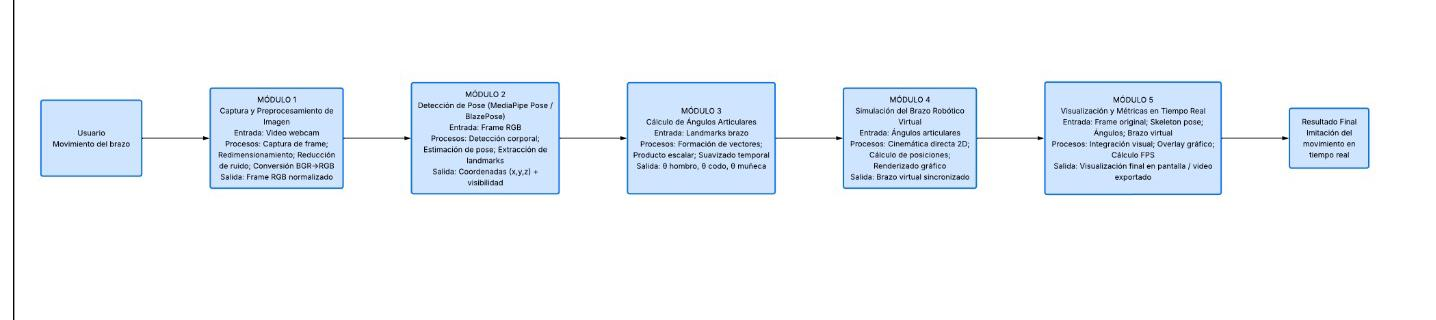
\includegraphics[width=1\textwidth]{images/diagrama_bloques.jpeg}
    \caption{Arquitectura conceptual del pipeline de procesamiento en tiempo real.}
    \label{fig:pipeline}
\end{figure}

\subsubsection*{Diseño del Módulo M3 -- Cálculo de Ángulos}

El módulo M3 implementa el cálculo de ángulos mediante la siguiente
lógica para cada articulación:

\begin{enumerate}
    \item Extraer las coordenadas 2D $(x, y)$ en píxeles de los landmarks
          proximal, central y distal de la articulación.
    \item Construir los vectores $\vec{v}_1$ (de central a proximal) y
          $\vec{v}_2$ (de central a distal).
    \item Calcular el ángulo mediante la ecuación \ref{eq:angulo_s2}:
          \begin{equation}
              \theta \;=\; \arccos\!\left(
                \frac{\vec{v}_1 \cdot \vec{v}_2}
                     {|\vec{v}_1|\,|\vec{v}_2|}
              \right)
              \label{eq:angulo_s2}
          \end{equation}
          El resultado en radianes se convierte a grados.
    \item Aplicar filtro de media móvil de ventana $w = 5$ sobre el
          historial de ángulos de la articulación.
    \item Retornar el ángulo suavizado junto con un flag de validez
          (\texttt{True} si visibilidad de todos los landmarks $>$ 0.5).
    \item Calcular la apertura del gripper: distancia euclidiana entre landmark 19 (punta índice) y landmark 21 (punta pulgar), normalizada entre un valor mínimo $d_{min}$ (pinza cerrada) y máximo $d_{max}$ (pinza abierta), expresada como porcentaje [0\%, 100\%].
\end{enumerate}

\subsubsection*{Diseño del Módulo M4 -- Cinemática Directa 2D}

El brazo robótico virtual se modela como una cadena cinemática de tres
eslabones más un efector final tipo gripper, anclada en una posición
fija de la pantalla (base). Las longitudes de eslabón son parámetros
configurables (en píxeles):

\begin{itemize}[leftmargin=1.5em]
    \item $L_{\text{hombro}} = 120$ px (eslabón 1: base $\to$
          articulación 1)
    \item $L_{\text{antebrazo}} = 100$ px (eslabón 2: articulación 1
          $\to$ articulación 2)
    \item $L_{\text{mano}} = 60$ px (eslabón 3: articulación 2
          $\to$ efector final)
    \item $L_{\text{gripper}} = 30$ px por rama (dos segmentos
          divergentes que representan la apertura de la pinza;
          el ángulo entre ellos es proporcional a
          $a_{\text{gripper}}$ calculado en M3)
\end{itemize}

Las posiciones cartesianas de cada junta se calculan mediante cinemática
directa acumulativa (ecuaciones \ref{eq:cinematica_s2}):

\begin{align}
  x_1 &= x_0 + L_{\text{hombro}}\cos(\theta_{\text{hombro}})
  \notag \\
  y_1 &= y_0 - L_{\text{hombro}}\sin(\theta_{\text{hombro}})
  \notag \\
  x_2 &= x_1 + L_{\text{antebrazo}}
               \cos(\theta_{\text{hombro}} + \theta_{\text{codo}})
  \notag \\
  y_2 &= y_1 - L_{\text{antebrazo}}
               \sin(\theta_{\text{hombro}} + \theta_{\text{codo}})
  \label{eq:cinematica_s2}
\end{align}

\subsection{Bocetos y Flujos de Pantalla}

A continuación se describen los bocetos del sistema y los flujos de
pantalla principales. Los bocetos representan la disposición visual de
la interfaz de usuario en la ventana de visualización de OpenCV.

\subsubsection*{Boceto 1 -- Pantalla Principal (Vista en tiempo real)}

La ventana principal muestra el frame de video (640$\times$480 px) con
los siguientes elementos superpuestos:

\begin{figure}[H]
    \centering
    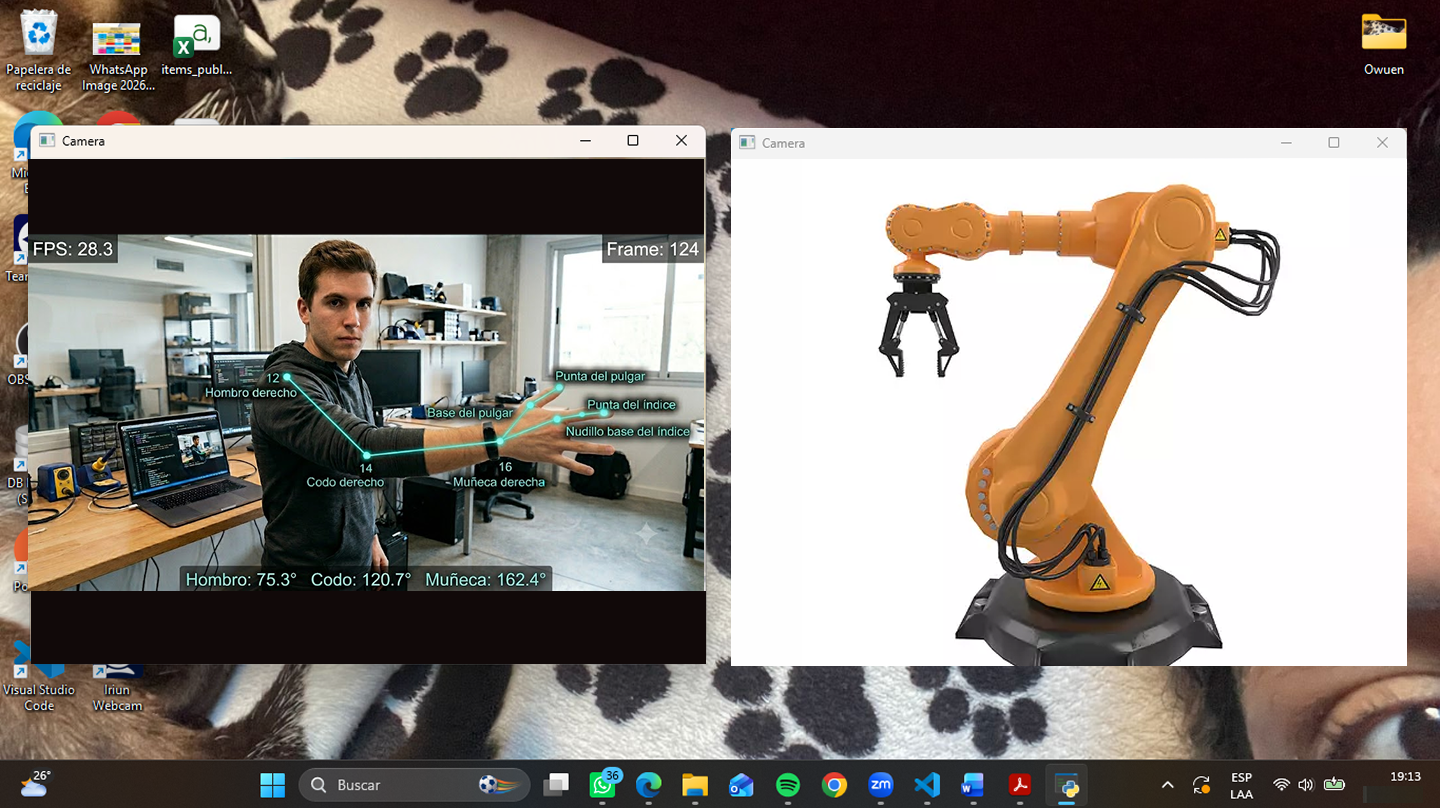
\includegraphics[width=0.75\textwidth]{images/boceto_pantalla.png}
    \caption{Boceto de la pantalla principal del sistema (ventana OpenCV en
             tiempo real). Elementos: contador FPS, número de frame,
             skeleton MediaPipe con landmarks,  brazo robótico
             virtual, ángulos articulares
             calculados en tiempo real.}
    \label{fig:boceto_pantalla}
\end{figure}

\subsubsection*{Boceto 2 -- Flujo de Pantalla del Sistema}

El flujo de interacción del usuario con el sistema sigue la secuencia
de estados de la figura \ref{fig:flujo_pantalla}.

\begin{figure}[h!]
    \centering
    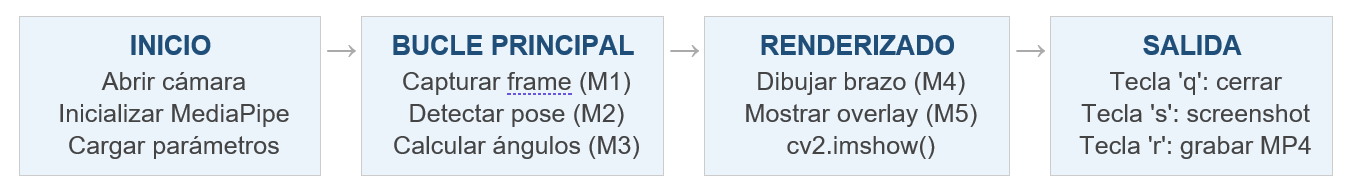
\includegraphics[width=1\textwidth]{images/flujo_pantalla.png}
    \caption{Flujo de pantalla del sistema}
    \label{fig:flujo_pantalla}
\end{figure}

% ============================================================
\section{Plan de Implementación del Proyecto}
% ============================================================

El plan de implementación sigue la metodología SCRUM con tres sprints.
El Sprint \#1 (semanas 1--2) cubrió la definición del problema. El
Sprint \#2 (semanas 3--4) cubre la metodología. El Sprint \#3
(fin del curso DIP) abarca el desarrollo completo, análisis de resultados y
conclusiones. \cite{Vintimilla2026}

\begin{table}[H]
\centering
\label{tab:plan_impl}
\renewcommand{\arraystretch}{1.3}
\begin{tabularx}{\textwidth}{
    >{\bfseries}p{1.5cm}
    p{1.6cm}
    X
    p{3.5cm}
}
\toprule
\textbf{Sprint} &
\textbf{Semanas} &
\textbf{Actividades principales} &
\textbf{Entregable} \\
\midrule
Sprint \#1 & 1--2 &
  Revisión del estado del arte (tema macro, componentes y herramientas).
  Definición del diagrama de bloques y módulos. Definición de objetivos,
  entradas y salidas por módulo. &
  Informe \#1 (Secciones 1.1--1.5) \\
\midrule
Sprint \#2 & 3--4 &
  Análisis de datos (datasets, características, preprocesamiento).
  Análisis de confiabilidad y compatibilidad. Definición de
  requerimientos, recursos, diseño conceptual y bocetos. Plan de
  implementación. &
  Informe \#2 (Sección 2) \\
\midrule
Sprint \#3 -- Fase 1 & 5--7 &
  M1: captura y preprocesamiento (cv2.VideoCapture, normalización,
  filtro gaussiano). M2: integración MediaPipe Pose y extracción de
  landmarks 11--16. M3: cálculo vectorial de ángulos con filtro media
  móvil y pruebas unitarias. Incluye cálculo de apertura del gripper por distancia euclidiana landmarks 19–21. &
  Código M1--M3 funcional + pruebas unitarias \\
\midrule
Sprint \#3 -- Fase 2 & 8--10 &
  M4: cinemática directa 2D, renderizado del brazo y simulación visual del gripper (apertura/cierre). M5:
  visualización integrada y FPS overlay. Integración de M1--M5 en
  pipeline completo. &
  Sistema integrado funcional a $\geq$ 20 FPS \\
\midrule
Sprint \#3 -- Fase 3 & 11--12 &
  Evaluación del sistema: FPS, MAE angular, robustez ante iluminación.
  Análisis estadístico con scikit-learn y gráficas con matplotlib.
  Redacción de conclusiones, recomendaciones y futuros trabajos. &
  Informes \#3 y \#4 (Secciones 3 y 4) \\
\bottomrule
\end{tabularx}
\caption{Plan de implementación del proyecto por sprint y semanas.}
\end{table}

\subsection{Gestión de Riesgos}

Se identifican los siguientes riesgos técnicos con sus planes de
mitigación:

\begin{table}[H]
\centering
\label{tab:riesgos}
\renewcommand{\arraystretch}{1.3}
\begin{tabularx}{\textwidth}{
    X
    p{2cm}
    p{1.8cm}
    X
}
\toprule
\textbf{Riesgo} &
\textbf{Probabilidad} &
\textbf{Impacto} &
\textbf{Mitigación} \\
\midrule
FPS $<$ 20 en hardware de bajo rendimiento &
  Media & Alto &
  Reducir resolución a 320$\times$240; desactivar skeleton completo;
  usar MoveNet como fallback \\
\midrule
Oclusión del brazo en poses extremas &
  Alta & Medio &
  Implementar umbral de visibilidad ($>$ 0.5); mantener último ángulo
  válido cuando visibilidad es baja \\
\midrule
Ruido excesivo en landmarks por iluminación deficiente &
  Media & Medio &
  Aumentar ventana de media móvil a $w = 10$; Inversión de capital en mejorar condiciones de iluminación \\
\midrule
Incompatibilidad de versiones de librerías &
  Baja & Alto &
  Fijar versiones exactas en requirements.txt; usar entorno
  virtual Python aislado \\
\bottomrule
\end{tabularx}
\caption{Identificación de riesgos técnicos y planes de mitigación.}
\end{table}


%%%%%%%%%%%%%%%%%%%%%%%%%%%%%%%%%%%%%%%%%%%%%%%%%%%%%%%%%%%%%%%%%%%%%%%%%%%%%%%%%
%% Source defintions
%%%%%%%%%%%%%%%%%%%%%%%%%%%%%%%%%%%%%%%%%%%%%%%%%%%%%%%%%%%%%%%%%%%%%%%%%%%%%%%%%
% When no use outcommentBazarevskyetal2020
% !TeX root = ../alda_g17.tex

\bibliographystyle{ieeetr}

\renewcommand\bibname{References}
\bibliography{base/sources}


%%%%%%%%%%%%%%%%%%%%%%%%%%%%%%%%%%%%%%%%%%%%%%%%%%%%%%%%%%%%%%%%%%%%%%%%%%%%%%%%%
%% Inserting the appendix
%%%%%%%%%%%%%%%%%%%%%%%%%%%%%%%%%%%%%%%%%%%%%%%%%%%%%%%%%%%%%%%%%%%%%%%%%%%%%%%%%
% When no use outcomment
%% !TeX root = ../alda_g17.tex

\newpage
\appendix 
% Adds appendix as chapter to toc
\addcontentsline{toc}{chapter}{Appendix}


\chapter{First}


\chapter{Second}


\end{document}
